\documentclass[10pt,a4paper]{article}
\usepackage[natbibapa]{apacite} 
\usepackage{amsmath}
\usepackage{tikz}
\usepackage{physics}
\usepackage[a4paper,margin=1.2in]{geometry} 
\bibliographystyle{apacite}


\title{Assignment 3 Machine Learning COS4852}
\author{ Adriaan Louw (53031377) }

\tikzset{
  treenode/.style = {shape=rectangle, rounded corners,
                     draw, align=center,
                     top color=white, bottom color=blue!20},
  root/.style     = {treenode, font=\Large, bottom color=red!30},
  env/.style      = {treenode, font=\ttfamily\normalsize},
  dummy/.style    = {circle,draw}
}

\newcommand{\eeq}[1]{\begin{equation}
\begin{split}
#1
\end{split}
\end{equation}}

\usetikzlibrary{shapes.misc}
\usetikzlibrary{decorations.pathreplacing}
\usetikzlibrary{positioning}

\tikzset{cross/.style={cross out, draw=black, minimum size=20*(#1-\pgflinewidth), inner sep=0pt, outer sep=0pt}, 
%default radius will be 1pt. 
cross/.default={1pt}}


\tikzset{basic/.style={draw,fill=blue!50!green!20,
                       text badly centered,minimum width=3em}}
\tikzset{input/.style={basic,circle}}
\tikzset{weights/.style={basic,rectangle,minimum width=2em}}
\tikzset{functions/.style={basic,circle,fill=blue!50!green!20}}
\newcommand{\addsymbol}{\draw[thick] (0.5em,0.5em) -- (0,0.5em) -- 
                        (0,-0.5em) --  (-0.5em,-0.5em)
                        (0em,0.75em) -- (0em,-0.75em)
                        (0.75em,0em) -- (-0.75em,0em);}
\begin{document}

\maketitle

\tableofcontents

\section{Question 1}
Given Bayes' theorem where

\begin{equation}
P(A|B) = \frac{P(B|A)P(A)}{P(B)}
\end{equation}

We need to calculate the probability of Joe being a librarian (L) given that he has glasses. (G) This can be expressed as follows using Bayes' theorem from above

\begin{equation}
P(L|G) = \frac{P(G|L)P(L)}{P(G)}
\end{equation}

We know that $P(G|L)$ is the probability that a librarian is wearing glasses, $P(L)$ is the probability that a man is a librarian an $P(G)$ is just the probability of a man wearing glasses. These probabilities are provided. Thus putting them into the above equation gives

\begin{equation}
\begin{split}
P(L|G) &= \frac{P(G|L)P(L)}{P(G)}\\\\
       &= \frac{(1)(\frac{1}{12000})}{0.12}\\
       &= 0.00069
\end{split}
\end{equation}

The probability that Joe is a librarian is 0.00069

Following the same argument we need to determine the probability that Joe is a salesman (S) given that 
he wears glasses. Using Bayes' theorem  again we have

\begin{equation}
P(S|G) = \frac{P(G|S)P(S)}{P(G)}
\end{equation}

$P(G|S)$ is the probability that a salesman wears glasses. $P(S)$ is the probability that a man is a salesman and $P(G)$ is again the probability that a person wears glasses. We are given this information. We now work out $P(S|G)$

\begin{equation}
\begin{split}
P(S|G) &= \frac{P(G|S)P(S)}{P(G)}\\
       &= \frac{(\frac{1}{25})(\frac{1}{200})}{0.12} \\
       &= 0.00166
\end{split}
\end{equation}

We find that it is much more likely for Joe to be a salesman than a librarian. This is not what we would expect. We would expect for him to be a librarian given that every librarian wears glasses. Without more information there is no better way to calculate whether Joe is a librarian or a salesman.  
\section{Question 2}
\subsection{Question 2a}

The network has 5 nodes namely Smoker (named variable S), Lung Cancer (named variable C), Pollution (named variable P), X-Ray (named variable X) and Dyspnoea (named variable D). Refer to Figure \ref{fig}.
 
Smoker (S) has 2 states: Yes (y) and No (n)

Lung Cancer (C) has 2 states: True (t), False (f)

Pollution (P) has 2 states: High (h) and low (l)

X-Ray has 2 states: Abnormal (a) and Normal (n)

Dyspnoea has 2 states: Present (p) and Absent (a)

Lung Cancer is dependant on Smoker and Pollution. While X-Ray and Dyspnoea is dependant on Lung Cancer. This relationship can be seen in Figure \ref{fig}.

\subsection{Question 2b}
The bayesian network is described by Figure \ref{fig}

\begin{figure}
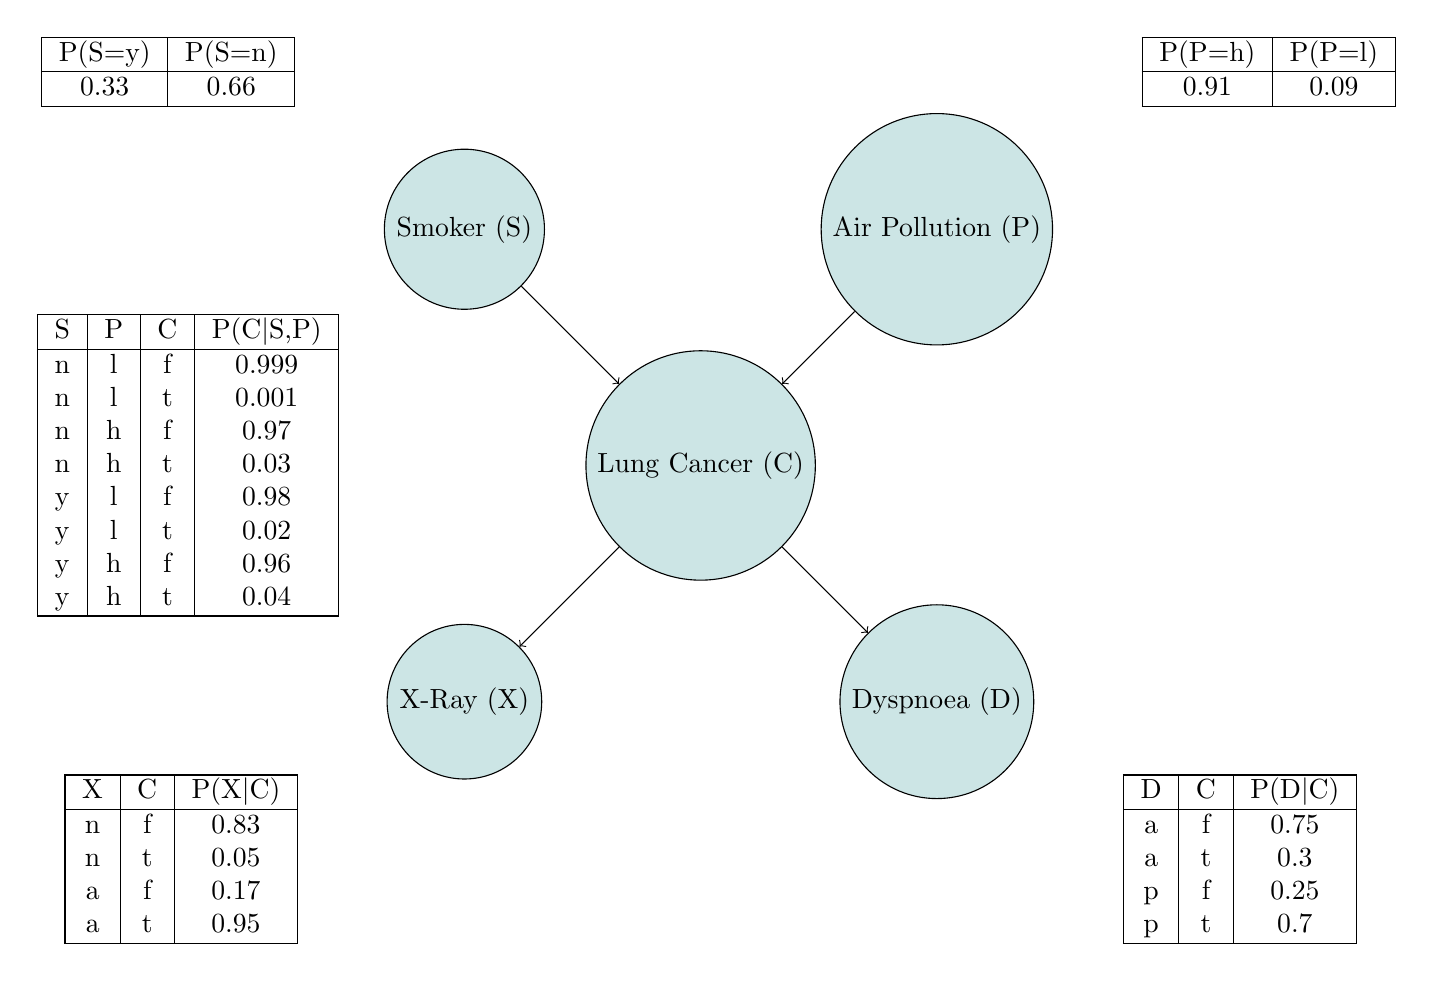
\begin{tikzpicture}[scale=1.0]

    \node[input] (s) at (-3,3){Smoker (S)};
    \node[input] (a) at (3,3){Air Pollution (P)};
    
    \node[input] (l) at (0,0){Lung Cancer (C)};
    
    \node[input] (x) at (-3,-3){X-Ray (X)};
    \node[input] (d) at (3,-3){Dyspnoea (D)};
    
    
    \draw[->] (s) -- (l);   
    \draw[->] (a) -- (l);
    \draw[->] (l) -- (x);
    \draw[->] (l) -- (d);
    
    \node[left=of s,yshift=2cm](smoker) {%
    	\begin{tabular}{|c|c|}
    	\hline
    	P(S=y)  & P(S=n)\\
    	\hline
    	0.33 & 0.66\\
    	\hline
    	\end{tabular}
    };   
    
    \node[right= of a,yshift=2cm](pollution){
		\begin{tabular}{|c|c|}
		\hline
		P(P=h) & P(P=l)\\
		\hline
		0.91 & 0.09 \\
		\hline
		\end{tabular}		    
    }; 
    
    \node[left= of l,yshift=0cm, xshift=-2cm](cancer){
		\begin{tabular}{|c|c|c|c|}
		\hline
		S & P & C & P(C$|$S,P)\\
		\hline
		n & l & f & 0.999  \\
		n & l & t & 0.001 \\
		n & h & f & 0.97 \\
		n & h & t & 0.03 \\
		y & l & f & 0.98 \\
		y & l & t & 0.02 \\
		y & h & f & 0.96 \\
		y & h & t & 0.04 \\
		\hline
		\end{tabular}		    
    }; 
    
    \node[left= of x, yshift=-2cm](xray){
    	\begin{tabular}{|c|c|c|}
    	\hline
    	X & C & P(X$|$C) \\
    	\hline
    	n & f & 0.83 \\
    	n & t & 0.05 \\
    	a & f & 0.17 \\
    	a & t & 0.95 \\
    	\hline
    	\end{tabular}
    };
    
    \node[right= of d, yshift=-2cm](dyspnoea){
    	\begin{tabular}{|c|c|c|}
    	\hline
    	D & C & P(D$|$C) \\
    	\hline
    	a & f & 0.75 \\
    	a & t & 0.3 \\
    	p & f & 0.25 \\
    	p & t & 0.7 \\
    	\hline
    	\end{tabular}
    };
    
    
\end{tikzpicture}
\caption{Bayesian Network}
\label{fig}
\end{figure}

\section{Question 3}

\end{document}
